\subsection{Trigger system of the LHCb experiment}

The LHCb experiment is operating in the forward region of LHC collisions and was originally designed to precisely study heavy-flavour decays involving $CP$ and flavour violation.
\todo[inline]{Add here citation to LHCb TDR}
Currently, the LHCb detector operates as a general-purpose forward detector with a broad physics program including e.g. dark matter searches and electroweak physics. 
The LHCb trigger system was redesigned for Run~3, removing the low-level Level 0 (L0) hardware-based trigger previously employed in Runs 1 and 2. 
\todo[inline]{Add here citation to LHCb Run-3 trigger paper}
At the Run~3 LHCb luminosity of about \SI{2e33}{\per\square\cm\per\second}, the maximum output rate of \SI{1}{\mega\hertz} of the L0 trigger and its simple selection criteria based on transverse momenta would result in a saturation of the yields of several processes as seen in Figure~\ref{fig:LHCbL0TriggerYield}. 
\todo[inline]{It is not clear what this figure shows to someone not in LHCb, it needs to be described more both in text and in caption}

The upgraded LHCb trigger consists solely of a High-Level Trigger (HLT), split between two stages: HLT1 and HLT2~\cite{Aaij:2019uij}. Following the removal of the L0 trigger, LHCb event readout has increased from \SI{1}{\mega\hertz} to \SI{30}{\mega\hertz}\footnote{The LHCb Event Builder was designed to handle the average bunch crossing of 30 MHz, as well as the maximum crossing rate of 40 MHz.}. During Run~2, HLT1 and HLT2 were decoupled to allow HLT1 to run synchronous to data-taking and HLT2 to run asynchronously, enabling detector calibrations between the two steps to improve reconstruction performance to a quality previously only achieved offline~\cite{LHCb:Albrecht_2015}.
\todo[inline]{Add here citation to LHCb Run-3 trigger paper instead of older proceedings}


\begin{figure}[h!]
    \centering
    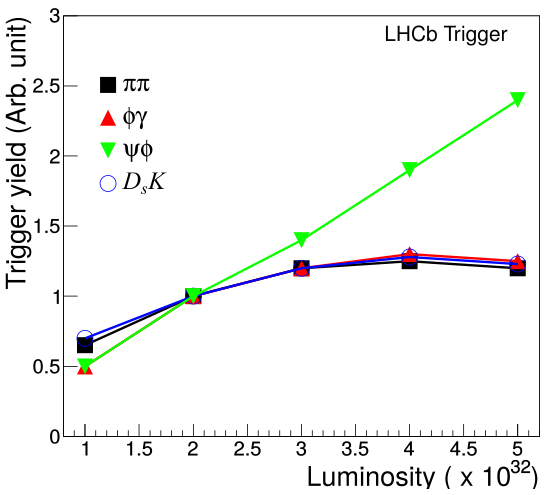
\includegraphics[width=0.55\linewidth]{images/lhcb/LHCb-L0-yield.png}
    \caption{Trigger yield per mode of interest as a function of the luminosity in ${\rm cm}^{-2}{\rm s}^{-1}$ with the Run 2 trigger configuration from Ref.~\cite{LHCb:upgrade-piucci}. Any increase in luminosity from accelerator upgrades is suppressed by the L0 trigger in most $B$ meson decay channels.}
    \label{fig:LHCbL0TriggerYield}
\end{figure}

HLT1 was upgraded to perform a partial reconstruction of the full detector readout. To achieve this, the reconstruction algorithms were upgraded to run on GPUs hosted on the same event-building servers that host the FPGA cards required to receive data from the detector at \SI{30}{\mega\hertz}~\cite{LHCb_Allen_GPU}. Reconstructed, selected events are propagated to a buffer at an event rate of ${\sim}\SI{1}{\mega\hertz}$. HLT2, implemented as a CPU farm known as the Event Filter Farm (EFF), takes as input the most recent detector alignment and calibration, reconstructing events in full offline quality for detailed selection. This selection reduces the output bandwidth to \SI{10}{\giga\byte\per\second}, corresponding to an event rate of $\sim\SI{100}{\kilo\hertz}$~\cite{lhcb_hlt2_storage_run3}.
